% math.tex

\chapter{Mathematical Preliminaries}

To extract biologically meaningful information from large data sets, researcher rely heavily on mathematical insights which
guarantee run time estimates, bounds on the problem domain, or interpretation of significance.  While studying the relationship
between chromatin topology and fragility, we leveraged several statistical and linearly algebraic tools.  The following section
will explain the underlying mathematical notions behind the algorithms, the biological rationale, and an interpretation of their
results.  We assume the reader is familiar with the mechanics of linear algebra, an elementary course in statistics, and numerical
analysis.  The reader is heartily encouraged to consult the references to gain a more complete understanding than possible to
present here.

\section*{Normalization of Chromatin Contact Maps}

The entry point for topological analysis begins with a chromatin \gls{contact map}.  The experimental procedure generating a chromatin
contact map, called a Hi-C experiment, is described in detail in Chapter 3.  For now, we will attempt to motivate our
analysis with a simple thought experiment.

Suppose that one wished to record the conformation of a string folded randomly on a surface.  In particular, suppose we focus on intersections
where two strands cross or lie in close proximity.  One possibility would be to place a one-dimensional coordinate system on the string, say
$0 \leq  x \leq  L, x \in \mathbb{N}$.  Since we are interested in overlapping regions, we refer to the region $X_i = \left[ x_{i}, x_{i+1}\right]$
as a bin.  We can record overlapping regions as pairs $(X_i,X_j)$, where position $X_i$ is in close proximity to position $X_j$.  The
coordinate pairs naturally form a graph, which we represent computationally as a matrix $\matr{O}$.  As $L \rightarrow \infty$, the
resolution of the matrix increases (bin sizes become smaller), and precise interactions on a smaller scale can be differentiated.
Figure~\ref{fig:string} is an example of one such diagram.

\begin{figure}[b]
  \centering
  \caption{Example: Interactions on a String}
  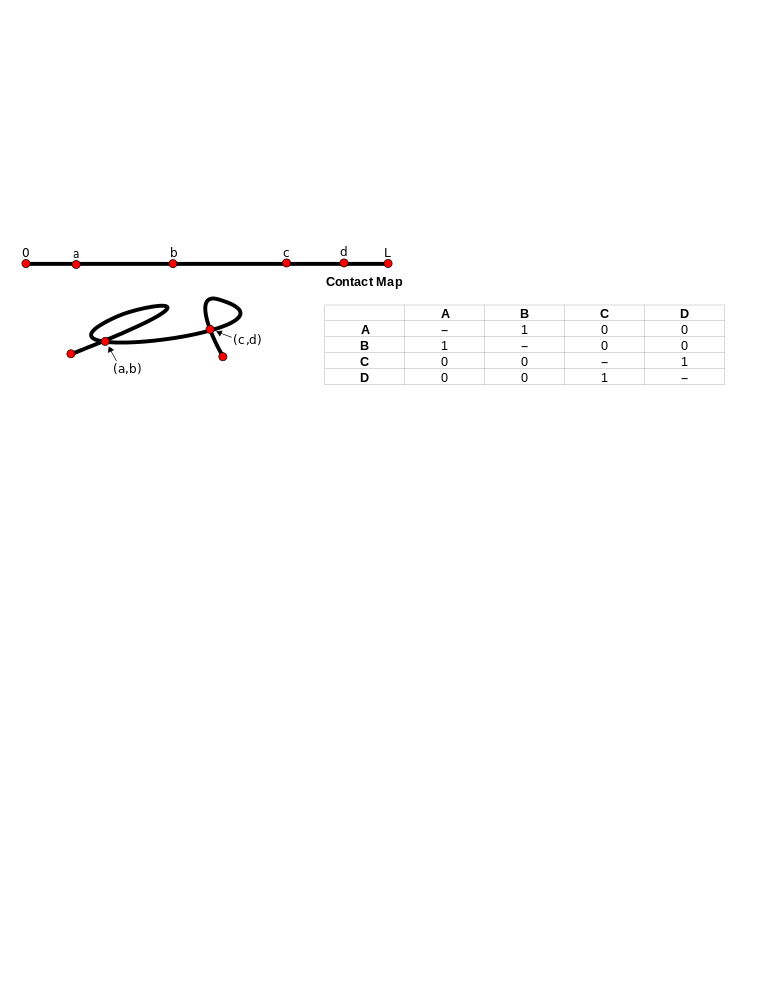
\includegraphics[width=\textwidth]{figures/mathematics/strmtx}\label{fig:string}
\end{figure}

The data structure produced by a Hi-C experiment is identical in spirit to the model developed in our thought experiment.  However, instead of
interactions occurring on a single string, the human genome consists of 24 independent chromosome `strings'.  Furthermore, interaction maps are
generated from populations of cells, yielding millions of copies of each genome.  With this in mind, we propose the following definition:

\begin{defn}
  A chromatin contact map $\matr{O}$ is a symmetric $N \times N$ matrix.  Each cell or bin $O_{ij}$ contains the number of observed contacts
  between regions $i$ and $j$ on the genome.  The contact map is a measure of the contact probability between loci on a genome-wide scale.
\end{defn}

Contacts are recorded by binning the genome into equally sized intervals and considering the pairwise interactions between each bin.
Typically, bins are ordered by increasing genomic coordinates, from the first bin of chromosome 1 to the last bin of chromosome X.
Depending on data quality, bin sizes range from tens of kilobases to megabases.

The critical step of any data analysis pipeline is data \gls{normalization}, which removes experimental biases and noise.  Coupled with quality
control measurements and experimental replicates, normalization also establishes a level of reproducibility.
Several methods exist to normalize contact maps.  Tanay and Yaffe were among the first researchers to undertake a statistical analysis of the
Hi-C experiment in 2011 \citep{yaffe2011}.  They identify several sources of systematic experimental bias in the Hi-C assay and propose a
probabilistic background model that computes the probability of \glspl{trans contact} and \glspl{cis contact} based on regional
\gls{GC} content, fragment length, and genome mappability.  Corrected contact maps are calculated by solving the maximum-likelihood model
parameters on model contact maps, which are then applied to the experimentally derived contact maps.  The mappings
achieved using Tanay and Yaffe's methods provide robust reproducibility between replicates and experiments by considering
\glspl{trans contact} and \glspl{cis contact} separately \citep{yaffe2011}.  This requirement renders their analysis computationally
intensive, prompting further research into simpler methods for Hi-C analysis.

Alternative methods have been developed to normalize contact maps.  Hu and colleagues propose a method `HiCNorm' based on Poisson
regression and achieve a $9000$-fold speed increase compared to Tanay and Yaffe's method \citep{hu2012}.  Recently, Ay and colleagues provide a statistical
method `Fit-Hi-C' that does not assume a particular underlying statistical distribution, instead normalizing \glspl{cis contact} based on probabilistic
analysis of polymer looping dynamics \citep{ay2014}.

Imakaev and colleagues propose a normalization and analysis pipeline \gls{ICE} \citep{imakaev2012}.  We employ \gls{ICE} as the normalization
algorithm in this thesis, due to the availability of its source code\footnote{source: \url{http://mirnylab.bitbucket.org/hiclib/}} and good
performance.  In the following section, we will discuss their algorithm in detail.

\subsection*{\glsentryfull{ICE}}

In pursuit of the true contact probability for each genomic region, \gls{ICE} makes a critical observation that the bias matrices determined by
Yaffe and Tanay \citep{yaffe2011} can be successfully reproduced ($r = 0.99$) as a product of biases $B_i \times B_j$.  This observation leads
immediately to the following proposition

\begin{prop}
  Given the assumption of factorizable biases, the expected contact frequency $\varepsilon_{ij}$ for every pair of regions $(i,j)$ can
  be written as $\varepsilon_{ij} = B_{i}B_{j}T_{ij}$, where $B_i$ and $B_j$ are biases and $T_{ij}$ is the sought matrix of relative contact
  probabilities, normalized as $\sum_{i, i \neq j, j \pm 1}T_{ij} = 1$.  The normalized contact map is give as
  $T_{ij} = \frac{\varepsilon_{ij}}{B_{i}B_{j}}$.
\end{prop}

The authors note that this normalization procedure results in `equal visibility' regions across the entire genome and maps which are
comparable between Hi-C data sets.  They propose the following algorithm to obtain the biases $B_i$ and `true' relative contact probabilities
$T_{ij}$.

\begin{algorithm}[H]
  \KwData{A matrix of observed interactions $O_{ij}$}
  \KwResult{A matrix of relative contact probabilities $T_{ij}$ and bias vector $B_i$}
  Initialize $W^{0}_{ij} = raw contact matrix$; $B^0 = 1$; $k = 1$\;
  \While{$\abs{B^{k+1} - B^{k}} < \delta$}{%
    $S_i = \sum_{j}W^{k}_{ij}$\;
    $\mean{S_i} = \frac{1}{n}\sum_{i = 1}^{n}S_i$\;
    $\Delta{}B^k_i = \frac{S_i}{\mean{S_i}}$\;
    $W^{k+1}_{ij} = \frac{W^k_{ij}}{\Delta{}B^k_i\Delta{}B^k_j}$\;
    $B^{k+1}_i = B^k_i \dot \Delta{}B^k_i$\;
    $k = k + 1$\;
  }
  \caption{Iterative Correction}
\end{algorithm}

It is not apparent that this algorithm is correct or even converges.  To gain an intuitive understanding of the solution, let us investigate a
simpler proposition.  Suppose that, instead of defining $O_{ij}$ to be the matrix product $B_{i}B_{j}T_{ij}$, we consider the counts
in $O_{ij}$ are the expectation of some multinomially distributed random variable $X_{ij}$, where $E[X_{ij}] = NB_{i}B_j$ for some
constant $N$ and vector $B$ whose cumulative sum is 1 ($\sum_{i}B_i = 1$).  In this formulation, we relax our criteria such that each cell
$O_{ij}$ is independent and distributed according to $B$.  The count of cell $i,j$ is given by the probability

\begin{align}
  \label{eqn:probmodel}
  \begin{split}
    p_{ij} &= NB_{i}B_{j}
    \\
    \log{p_{ij}} &=  c + u_i + u_j - Z
  \end{split}
\end{align}

where $c = \log{N}, u_i = \log{B_i}, u_j = \log{B_j}$, and $Z (= c)$ is a normalization factor to ensure that $\sum p = 1$.  This type of
model is called a \gls{log-linear} or \gls{toric model}.  $p$ is an observation from some distribution $p \sim \mathcal{f}(X)$.  The challenge to
parameterize the model and fit the model to the observed map.  The problem one of \gls{MLE}: what are the maximum likelihood parameters
that best fit the model to the observed data?  Fortunately, methods and their convergence properties for solving \glspl{MLE} have been extensively
studied in the literature \citep{fienberg2012, pachter2005}.

% TODO
In the realm of statistics, the contact matrix, together the vector sums of the rows and columns (margins), is called a \gls{contingency table}.  Assuming
that the margins are positive, and that the matrix cannot be permuted into block diagonal shape, Birch's theorem guarantees that there is a
unique maximum to the likelihood function \citep{pachter2005,bishop1975}.  For full details, consult Discrete Multivariate Analysis by
Bishop \citep{bishop1975}.  Furthermore, the marginal values are the \glspl{sufficient statistic} of the model.  In other words, the maximum
likelihood parameters for this data is given by the normalized row and column sums of the matrix \citep{pachter2005}.

With the observation that there exists a global maximum of the likelihood function, all that remains is to compute the true values by some
process.  One common algorithm is the \gls{EM} algorithm \citep{fuchs1982}.  Imakaev and colleagues employ a simpler algorithm known as \gls{IPF},
developed by Deming and Stephan in 1940, and apparently rediscovered by Imakaev's group \citep{deming1940}.  \gls{IPF} works generally by solving
the \gls{MLE} problem while leaving the margins ($p_{i+} = \sum_{j}p_{ij}$ and $p_{j+} = \sum_{i}p_{ij}$) fixed.  A proof of convergence for contingency
tables follows from Fienberg's work in algebraic geometry in 1970 \citep{fienberg1970}. %TODO explain feinburg more

Finally, we return to the \gls{toric model} we described in Eqn.~\eqref{eqn:probmodel}.  Since the log-likelihood function is concave, the \gls{IPF} algorithm first
computes the roots of the partial derivatives of the log-likelihood function and sets them to zero to solve for the global maximum.  Imakaev
and colleagues consider the likelihood function on the Poisson distribution, given by the \gls{pdf} $f(O;E) = \frac{E^{O}}{O!e^{-E}}$.  The
log-likelihood function for the Poisson distribution is given

\begin{align}
  \label{eqn:llmodel}
  LL = \sum_{ij}\left[O_{ij}\log{(T_{ij}B_{i}B_{j})} - T_{ij}B_{i}B_{j} - \log{(O_{ij}!)}\right]
\end{align}

Differentiating with respect to $T_{lm}$ and $B_m$ and setting the derivatives to zero yields

\begin{multicols}{2}
  \begin{align}
    \label{eqn:modelderivative1}
    \begin{split}
      \frac{dLL}{d\matr{T}_{lm}} = \frac{O_{lm}}{T_{lm}} - B_{l}B_{m} = 0
      //
      \frac{dLL}{dB_{m}} = \sum_i\left[\frac{\matr{O}_{im}}{B_m} - T_{im}B_i\right] = 0
    \end{split}
  \end{align}

  \break%

  \begin{align}
    \label{eqn:modelderivative2}
    \begin{split}
      T_{lm} = \frac{\matr{O}_{lm}}{B_{l}B_{m}}
      \\
      \sum_i\left[\frac{\matr{O}_{ij}}{B_{m}B_{i}} - \matr{T}_{im}\right]
    \end{split}
  \end{align}
\end{multicols}

It is clear that Eqn.~\eqref{eqn:modelderivative2} is satisfied if a solution is found for Eqn.~\eqref{eqn:modelderivative1}.  Taking the first equation together  with the
normalization $T_{ij}$ yields

\begin{align}
  \label{eqn:result}
  \sum_i \frac{\matr{O}_{ij}}{B_{i}B_{j}} = 1
\end{align}

A similar process yields that a broad class of distributions give the same result \citep{imakaev2012}.

\section*{Principal Component Analysis}

The holy grail of data analysis on high-dimensional data is dimensionality reduction --- that is, to find an accurate representation of
the experiment that need not invoke all the dimensions measured.  This is often performed as a preprocessing step to increase storage capacity
and algorithm speed.  Since experiments such as Hi-C produce data on large numbers of features, researchers must find ways to remove redundancy,
eliminate unneeded parameters and compress data sets.  One of the most popular methods is called \gls{PCA} \citep{law1987}.

Data in high dimensions are difficult to visualize and interpret.  Two common questions in data analysis are `what changed?' and `what
remained the same?' between measurements.  \gls{PCA} answers these questions by finding a representation of the data that maximizes
the \gls{variance} or variation between observations in the data set.  The output of \gls{PCA} is a transformed data set on a new coordinate
system, called components.  The \glspl{PC} are a subset of these components that capture `most' of the variation in the data set.  The researcher
must compare the calculated components to the original data set and determine which variables, or combination thereof, the components represent.

\begin{defn}[Principal Component Analysis]
  A statistical procedure that transforms a number of possibly correlated variables into a smaller number of uncorrelated variables.
\end{defn}

In practice, there are two methods used for \gls{PCA}.  The simplest to explain, but more error-prone, is the eigen-decomposition
method \citep{smith2006}.  In this procedure, for a data matrix $\matr{A}$, the eigenvalues of the covariance matrix $\matr{A}\matr{A}^T$
are computed directly as the principal components.  However, since this method requires an extra matrix multiplication, numerical
errors are more likely to be introduced during large computations. In practice, \gls{PCA} often derived in conjunction with \gls{SVD}
and we will hold to that standard here.

\begin{thm}[Singular Value Decomposition]
  Let $\matr{A} \in M_{n}(\mathbb{R})$ be given. Then there are unitary matrices $\matr{V} \in M_n$ and $\matr{W} \in M_n$, and a square diagonal
  matrix
  \[
    \matr{\Sigma} =
      \begin{bmatrix}
        \sigma_1 &        & 0        \\
                 & \ddots &          \\
        0        &        & \sigma_n \\
      \end{bmatrix}
  \]
  such that $\sigma_1 \geq \sigma_2 \geq \cdots \geq \sigma_n$ and $\matr{A} = \matr{V}\matr{\Sigma}\matr{W}^*$.  The parameters $\sigma_1$,
  $\hdots$, $\sigma_n$ are the positive square roots of the decreasingly ordered non-zero eigenvalues of $\matr{A}\matr{A}^*$, which are the
  same as the decreasingly ordered nonzero eigenvalues of $\matr{A}^*\matr{A}$.
\end{thm}

To prove that any square matrix $\matr{A} \in M_n(\mathbb{R})$ can be decomposed into singular values, we will use some matrix definitions. The
reader is reminded of the definitions of \textit{normal} $(\matr{A}\matr{A}^* = \matr{A}^*\matr{A})$, \textit{Hermetian} $(\matr{A}^* =  \matr{A})$,
and \textit{unitary} $(\matr{A}^*\matr{A} = \matr{A}\matr{A}^* = 1)$ matrices.  Further, two matrices $\matr{A}, \matr{B} \in M_n$ are said to be
\textit{unitarily similar} they are similar by a unitary matrix $(\matr{A} = \matr{U}\matr{B}\matr{U}^*)$.  We are now ready to begin the proof.

\begin{proof}[Singular Value Decomposition]
  It should be clear the matrices $\matr{A}\matr{A}^* \in M_n$ and $\matr{A}^*\matr{A} \in M_n$ have the same eigenvalues, and hence, they are
  unitarily similar.  Then there exists a unitary matrix $\matr{U}$ such that $\matr{A}^*\matr{A} = \matr{U}(\matr{A}\matr{A}^*)\matr{U}^*$.  Then

  \[
    {(\matr{UA})}^*(\matr{UA}) =
    \matr{A}^*\matr{U}^*\matr{UA} =
    \matr{A}^*\matr{A} =
    \matr{UA}\matr{A}^*\matr{U}^* =
    \matr{UA}{(\matr{U}\matr{A})}^*
  \]

  so $\matr{UA}$ is normal.  Let $\lambda_1 = \abs{\lambda_1}e^{i\theta_1}, \ldots, \lambda_n = \abs{\lambda_n}e^{i\theta_n}$ be the positive eigenvalues of
  $\matr{UA}$ in decreasing order.  Furthermore, let $\Delta = diag(\lambda_1, \ldots, \lambda_n)$, let $D = diag(e^{i\theta_1}, \ldots, e^{i\theta_n})$,
  let $\Sigma = diag(\abs{\lambda_1}, \ldots, \abs{\lambda_n})$, and let $\matr{X}$ be a unitary matrix such that $\matr{UA} = \matr{X\Delta}\matr{X}^*$.  Then
  $D$ is unitary and

  \[
    \matr{A} = \matr{U}^*\matr{X}\Sigma\matr{D}\matr{X}^* = (\matr{U}^*\matr{X})\Sigma(\matr{D}\matr{X}^*)
  \]

  If we denote $\matr{V} = \matr{U}^*\matr{X}$ and $\matr{W} = \matr{X}\matr{D}^*$, we have our desired factorization, and
  $\sigma_j = \abs{\lambda_j}, j = 1, \ldots, n$.
\end{proof}

A full proof of \gls{SVD} for rectangular matrices can be found in Horn and Johnson \citep{horn2013}. The relationship between
\gls{SVD} and \gls{PCA} follows directly from the definition of \gls{SVD}.

\begin{thm}
  Let $\matr{A} = \matr{V}\matr{\Sigma}\matr{W}^*$ be the \gls{SVD} of an $n \times n$ dimensional matrix $\matr{A}$ and let

  \[
    \matr{C} = \frac{1}{n - 1}\matr{A}^*\matr{A}
  \]

  be the covariance matrix.  The eigenvectors of $\matr{C}$ are the same as the \textnormal{right singular vectors} of
  $\matr{\Sigma}$.
\end{thm}

\begin{proof}
  Compute
  \[
    \matr{A}^*\matr{A} =
    \matr{V\Sigma}\matr{W}^*\matr{W\Sigma}\matr{V}^* =
    \matr{V\Sigma\Sigma}\matr{V}^* =
    \matr{V}\matr{\Sigma}^2\matr{V}^*
  \]

  \[
    \matr{C} = \matr{V}\frac{\matr{\Sigma}^2}{n - 1}\matr{V}^*
  \]

  $\matr{C}$ is symmetric, and unitarily diagnolizable.  Hence, the eigenvectors of the covariance matrix $\matr{C}$ are the same as the
  matrix $\matr{V}$ (right singular vectors) and the eigenvalues of $\matr{C}$ can be computed directly from the singular values
  $\lambda_i = \frac{\sigma_i}{n - 1}$.
\end{proof}

The ordered eigenvectors are the \glspl{PC} we desire.  In exploratory data analysis, the variance captured by each \gls{PC} is found
by analyzing the relative sizes of the positive eigenvalues, typically in the form of a scree plot.  In the Hi-C capture experiment, Dekker
and colleagues \citep{dekker2012} focus on the component that captures genome `compartment character', the banding pattern of interactions
observed on Hi-C maps, regardless of captured variance.  In our case, the \gls{PCA} decomposition provides a measure of compartment character
for a given bin on the Hi-C map.

\section*{Detecting features in local chromatin interaction}

\gls{PCA} is a useful technique for identifying gross differences between data sets; however, the method is computationally infeasable for large
data sets.  For subtle changes of local chromatin structure on high resolution maps, Dixon and colleagues developed a measure of chromatin
association bias for each bin termed the \gls{DI} \citep{dixon2012}.  Intuitively, the \gls{DI} for a given region of chromatin gives the
relative `upstream' or `downstream' bias of the interactions involving a particular chromatin region.  Regions constrained between prominent
downstream biases followed by high upstream bias form pockets of interactions called topological domains~\cite{dixon2012}.

The basic premise of the \gls{DI} algorithm is simple.  For each bin along the genome, the algorithm calculates the number of upstream and downstream
interactions and assigns the normalized difference ($downstream - upstream$) as the \gls{DI} for that particular bin.  The index captures the
downstream or upstream bias of a genomic region. The formulation of the directionality index is given in the supplementary methods
of Dixon's paper \citep{dixon2012}

\begin{align}
  \label{eqn:di}
  DI = \left(\frac{B - A}{\abs{B - A}}\right)\left(\frac{{(A - E)}^2}{E} + \frac{{(B - E)}^2}{E}\right)
\end{align}

where $A$ is the number of upstream reads in a given window, $B$ is the number of downstream reads, and $E$ is the expected number of interactions under
the null distribution ($\frac{A + B}{2}$).  Dixon and colleagues apply the directionality index to examine 2Mb windows upstream and downstream on a
normalized 40kb resolution contact map.  From the \gls{DI} vector, they employ a \gls{HMM}, with the \gls{DI} as observations and labels `upstream bias',
`downsteam bias' or `no bias' to discover conserved domains on contact maps.  For the full mathematical formulation of the \gls{HMM}, see \citet{dixon2012}.
They concluded that the domain boundaries were conserved across human and mouse cell types, and may represent part of the fundamental organizing principles
 of the metazoan genome \citep{dixon2012}.
